\section{Hardware Setup}

\subsection{List of components}
Here is a (maybe incomplete) list of our used components:
\begin{itemize}
	\item wooden chassis , 40 cm x 35 cm
	\item 1 small wooden board (approx. 20 cm x 25 cm)
	\item 11.1 V battery with 5000 mAh
	\item 11.1 V battery with 3500 mAh
	\item 4 soft-wheels(diameter: aprox. 12 cm)each soft-wheel can take max. 3 kg. 
	\item 4 Ethernet-UART  connected to the switch
	\item 4 Pololu motors (max. power: 60 W @ 12,5 V and 5 A)
	\item 1 Board (IMX6 Sabre Lite)
	\item 4 H-bridges (dual channel but we only use one channel)
	\item 4 DE0-Nano-Boards (FPGA’s)
	\item 1 LAN switch
	\item 2 DC-DC-Converters
	\item 2 ultrasonic sensors
\end{itemize}

\subsection{Overview}

\begin{figure}[h]
	\center{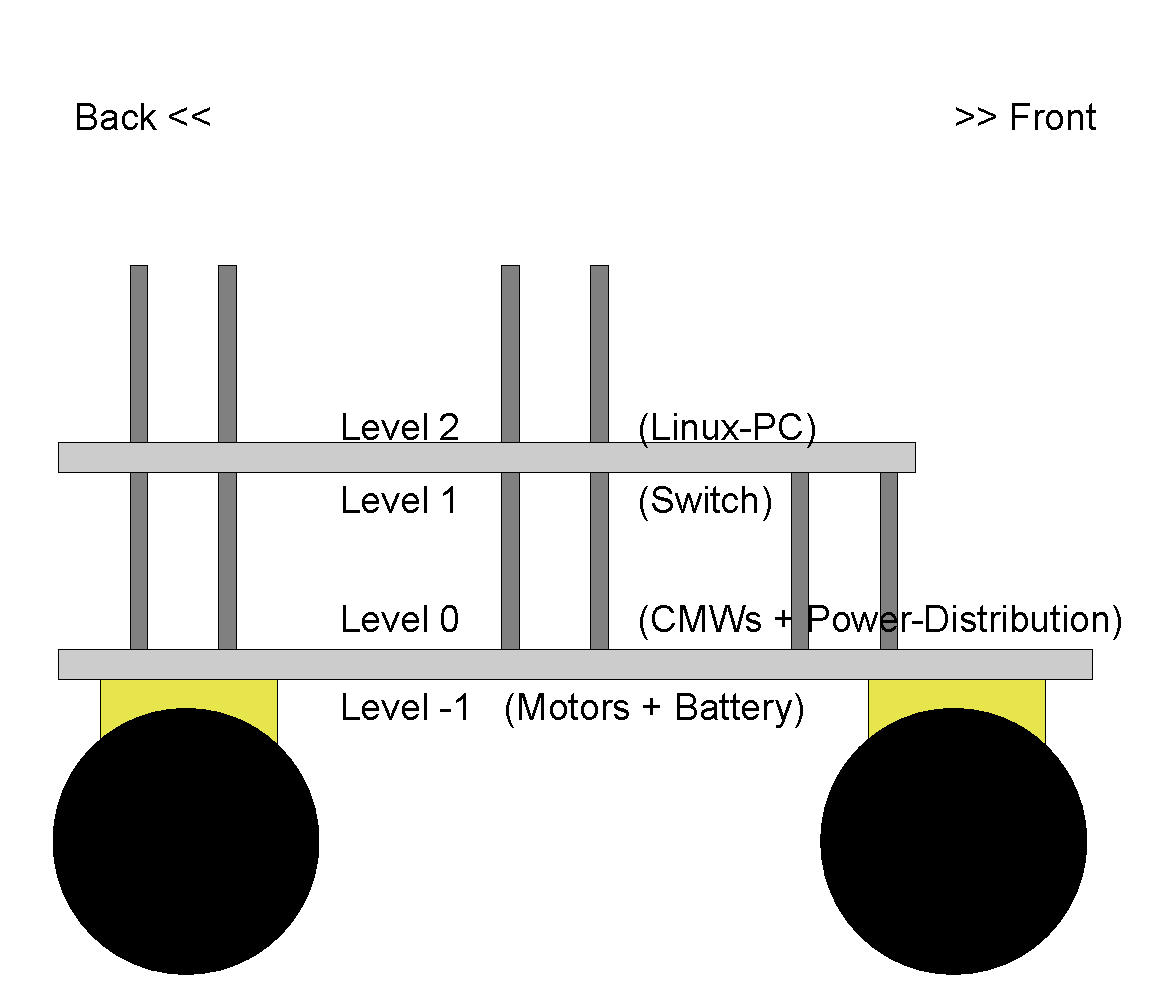
\includegraphics[width=0.5\textwidth]{figures/overview.pdf}}
	\caption{The car is divided into four levels. Each level has a different motto.}
\end{figure}

\subsection{Level -1}

\begin{figure}[ht] 
	\includegraphics[width=0.5\textwidth]{figures/level-1_b.jpg}
	\includegraphics[width=0.5\textwidth]{figures/level0_b.jpg}
	\caption{The lowest level -1 (see left figure) contains the four motors and the batteries. Level 0 (right figure) contains the four CMW-Units and the Voltage-Distribution.} \label{Level-1and0}
\end{figure}

The lowest level -1 (see \ref{Level-1and0}) contains the four motors and the batteries. Each motor is fixed on a small wooden block so the batteries are in a more safe place.

\subsection{Level 0}

The main level (see \ref{Level-1and0}) is the top of the wooden chassis. The power-distribution is fixed in the middle of the board and provides power to the H-bridges, the four FPGAs and the Linux-PC. The four H-bridges are placed in the corners. Next to each H-bridge there is the corresponding FPGA board. \\

At the back and front side of the car are ultrasonic sensors. They are fixed in an angle that the sensor measures the floor in 3.5 meters. Doing so gives us a maximum distance for reliable sensor values.\\

The next higher level sits down on 4 metal pillars fixed on the main level. 

\subsection{CMWUnit - Control-Motor-Wheel-Unit}
	Each Control-Motor-Wheel(CMW)-Unit consists of:
	\begin{itemize}	
		\item One \textit{Ethernet-UART} connected to the central FPGA
	
		\item One \textit{DE0Nano-Boards} (FPGA)
		
		\item One \textit{H-Bridge}	(dual-channel but we only use one channel)
	
		\item One \textit{Pololu Motor} (max. power: 60 W @ 12 V, 5 A).\\
		Problem: Many components can not take over 2 A! 
		
		\item One \textit{Soft-Wheel} (diameter: aprox. 12 cm)\\
		Problem: Each Soft-Wheel can take max. 3 kg 
	\end{itemize}
	
\begin{figure}[ht] 
	\center{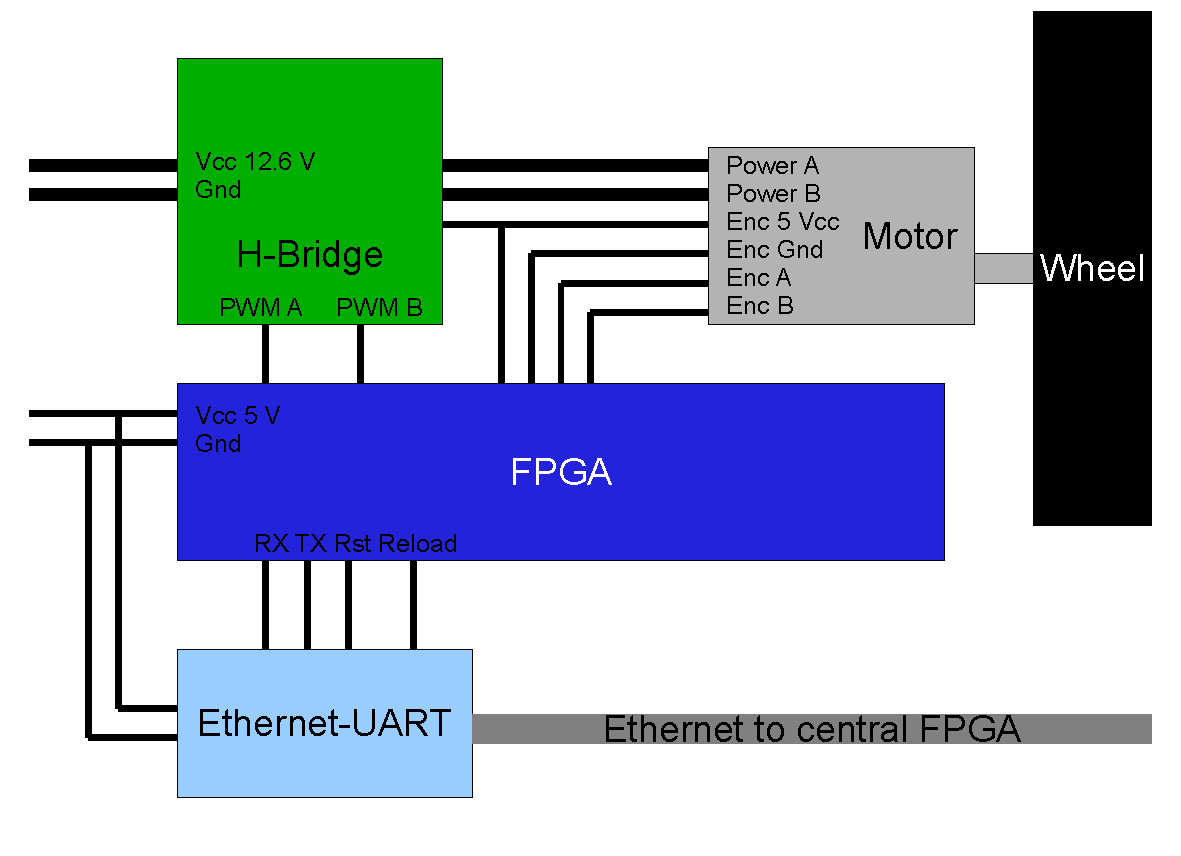
\includegraphics[width=0.5\textwidth]{figures/cmwunit.pdf}}
	\caption{Interconnections in the Control-Motor-Wheel-Unit} \label{CMWUnit}
\end{figure}

\subsection{Level 1}

\begin{figure}[ht] 
	\includegraphics[width=0.5\textwidth]{figures/level1_b.jpg}
	\includegraphics[width=0.5\textwidth]{figures/level2_b.jpg}
	\caption{Level 1 (see left figure) contains the Ethernet-Switch. Level 2 (see right figure) contains the (big) Sabre-light i.mx6 (Linux-PC).} \label{Level1and2}
\end{figure}

The small and light wooden board (see \ref{Level1and2}) is pillared by four metal sticks. From the button up there are 4 Ethernet-UART’s which are glued on the wood and connected by LAN-cables to the switch.\\

The switch is also fixed by glue on the wooden panel from the bottom up. To make it more solid the switch is first glued on a very small piece of wood and this is glued on the wooden panel.

\subsection{Level 2}

On the highest board (see \ref{Level1and2}) is the evaluation board (Linux-PC). Through a cut-out the evaluation board is connected with the switch on the other side. On the board are also pillars if someone would like to upgrade the car and build one more floor. For example fixing a camera or something similar on the top plank.
